\documentclass[12pt]{article}

\usepackage{float}
\usepackage{graphicx}
\graphicspath{ {./icons/} }

%Admin.gif:       GIF image data, version 89a, 39 x 39
%Cedo.gif:        GIF image data, version 89a, 40 x 40
%Frater.gif:      GIF image data, version 89a, 39 x 39
%Lib.gif:         GIF image data, version 89a, 39 x 39
%Mod.gif:         GIF image data, version 89a, 39 x 39
%Tech.gif:        GIF image data, version 89a, 39 x 39
%closedtopic.gif: GIF image data, version 89a, 400 x 322
%

\newcommand{\bnc}{{\textbf{Bolter \& Chainsword}}}%

\begin{document}

\tableofcontents
\listoffigures
\listoftables
\clearpage

\section{Introduction}

Welcome to the {\bnc}
\medskip

Before participating here, make sure that you have read the following 
rules; and make sure to follow them when you participate.
\medskip

All of the rules that follow are built upon the foundation of the 
mission statement and our principles. Note that many of our forums have 
additional guidelines (which are also built upon our mission 
statement), and you should be sure to read them also before posting.
\medskip

The most important thing to understand is the purpose of the {\bnc}
 as expressed in our mission statement:
\medskip

\subsection{Mission Statement}
\begin{quote}
The {\bnc} exists to help the members of a global hobby 
community to better understand, engage in, and enjoy all aspects of the 
Warhammer 40,000 hobby through constructive discussion and the sharing 
of hobby-related content.
\end{quote}


\subsection{Principles}

The principles by which the {\bnc} operates:

\begin{table}[H]
\begin{itemize}
\item We are all here united by our common enjoyment of the hobby.
\item We are all here as equals.
\item The differences between us neither define us nor divide us.
\item The differences make us stronger as individuals and as a 
community.
\item This site, this community, welcomes all hobbyists.
\end{itemize}
	\caption{The {\bnc} Principles}
\end{table}

\clearpage


%Basic Information (Allowed Content, Restrictions)
%Membership Rules (Accounts, Names, Avatars, Private Messages and 
%E-Mail, Membership Benefits)
%User Groups
%Signatures (Intent, Signature Content, Text, Images, Non-Compliance)
%Advertising
%Corrective Action
%Projects & Special Projects
%3D Printing
%Contacting the Administrators

\medskip

These rules are basic common sense stuff here folks and we don't think 
we are asking too much for everyone to follow them. If you have 
concerns or questions about any of the rules please contact the forum 
moderator(s), the custodes, or the administrators.
\medskip

Thanks!

\section{Basic Information}

The site is structured around the current edition of the Warhammer 
40,000 game, but all games set in the Warhammer 40,000 game universe 
are supported here.

In addition, while much of the core language used here is based around 
the core faction of Space Marines for which the site was first created, 
all factions of the Warhammer 40,000 game universe may be discussed 
here.

\subsection{Allowed Content}

The {\bnc} promotes constructive discussion about all 
aspects of the Warhammer 40,000 hobby. While the most recognizable 
content is the discussions, the term ``content'' applies to everything 
available here, including galleries, downloads, signatures, status 
updates, etc.

This is a public forum that is viewed by members from a wide range of 
age groups and cultural backgrounds. Please be considerate of others 
when composing your content (content includes posts, private messages, 
emails, reports, etc.). Appropriate topics include, but are not limited 
to:

\begin{figure}[H]
\begin{enumerate}
\item modeling and painting
\item army composition/list building
\item tactics and game play
\item rules queries
\item battle reports
\item background (also known as ``lore'' or ``fluff'')
\item official products (models, games, books, etc.)
\item Warhammer 40,000 and Games Workshop events
\item fan fiction and artwork
\item et cetera
\end{enumerate}
	\caption{List of appropriate topics and content.}
\end{figure}

\subsection{Restrictions}

Since our intent is for constructive discussion among fellow hobbyists 
from around the world and across all age groups, there are some 
restrictions in place to keep the forum a fun and safe place to discuss 
the hobby.

\subsubsection{No swearing/profanity}

Anything that can be said via swearing/profanity can be expressed in 
other terms, often far more articulately. Many words/terms are 
automatically filtered by the board software, replacing them with 
acceptable substitutes. Note that the ``no swearing/profanity'' rule 
includes all forms and mediums - written, oral (i.e., videos with 
audible profanity), visual (e.g., graphics with legible profanity) - 
and similarly includes abbreviations and substitutions (i.e., using 
alternate characters) as well as obscene gestures.
If you feel that swearing/profanity is the only way to accurately 
express yourself, a number of emoticons are available, especially 
``cuss'' emoticon {\texttt{:cuss:}}.

{\texttt{:cuss:}}

\subsubsection{No obscenity/pornography}

Sexually graphic content, whether written, audible, or visual, has no 
place here. Similarly, links to sexually graphic content are forbidden 
here. Posting obscenity/pornography or links to such content will 
subject you to summary banning from the site.
Note that there is room for some material that might be considered 
suggestive, generally where the followers of Slaanesh are concerned. 
Examples include some models and artwork (e.g., portrayals of 
daemonettes). The lines here are highly subjective, however, and 
discretion is advised. When in doubt, either don't post such material 
or contact an administrator/moderator first.
No disrespectful behavior (trolling, flaming, derogatory terms)

Trolling is being a jerk on the internet simply because you can. This 
is typically unleashing one or more cynical or sarcastic remarks on 
someone else, because it's the internet and, hey, you can (because they 
can't punch you in the face through the computer, even if you deserve 
it). Another form of trolling is posting material simply to provoke a 
negative response from others.
Flaming is engaging in or deliberately provoking heated argument 
online, usually involving personal attacks.
Derogatory terms are generally terms used to insult someone else, often 
on the basis of gender, sexual orientation, ethnicity, nationality, 
spiritual/religious beliefs, etc.
None of these types of behaviors are conducive to constructive 
discussion. There are going to be times when you disagree with someone 
and/or when you dislike someone or something, but you either need to 
express yourself constructively or you need to ignore/stay out of the 
discussion.

You don't have to actually respect everyone and everything, but you 
must treat them with respect here at the {\bnc}.

Just remember Wheaton's Law and live by it. :wink:

\subsubsection{No foreign languages or chat/``leet'' speak}

Our members come from around the world and all age groups. The intent 
of discussion here is for everyone to be able to participate. This site 
is an English language site (we don't all talk good English, mind you 
:wink: ). Using foreign languages or things like chat/``leet'' speak 
prevent many of our members from understanding, so they are not 
allowed. We don't expect perfect English, however, so please be 
understanding. Conversely, be tolerant of different styles of 
communication. Some of us are simply more blunt than others, and this 
is sometimes due to cultural norms (especially those of us from low 
context societies) and not necessarily because we're jerks.

\subsubsection{No spamming}

Spam isn't simply multiple identical posts across the forums, it also 
includes pointless, off-topic or smart-alec posts anywhere on the 
board. Remember, the {\bnc} is here to promote constructive discussion of 
the 40K hobby and anything not contributing to this may be considered 
spam and deleted. Repeat offenders may also be subject to corrective 
action for such behaviour.

\subsubsection{No trading or selling posts}

Trading and selling aren't bad in and of themselves, but we don't want 
the drama that comes when trades or sales go bad.

The exception to the above is that members may identify sales/trade 
offerings via their signatures, allowing follow-on contact via PM or 
e-mail. The {\bnc} accepts no responsibility or liability for such 
transactions, however.

\subsubsection{No intellectual property (IP) violations}

We enforce whatever Games Workshop allows with regard to usage of their 
IP. This applies to all Games Workshop products and subsidiaries. Refer 
to Games Workshop's website for their IP guidance.

Where third parties are concerned, we will similarly enforce whatever 
they provide with regard to using their IP. Again, refer to their sites.

When in doubt, less is better.

\subsubsection{No software cracks}

Whether requested or offered, software cracks are expressly forbidden 
here. This applies to any form of Warez or illegal downloading of any 
software, but particularly that related to GW Games will result in an 
immediate ban on your account.

\subsubsection{No excessive points values in army lists or discussions}

This means that you may not post Army Builder print outs (or those from 
similar products) or fully detailed points/stats for your army lists. 
Keep it simple, such as ``Chapter Master; Terminator armour, storm 
bolter, thunder hammer; 285 pts'' or similar.

\subsubsection{No off topic discussions}

We're here to discuss the hobby, not politics, nationalism, religion, 
sexuality or moral/ethical debates (or cars, or sports, or the latest 
movie, etc.).

\subsection{Disruptive behavior}

Disruptive behavior, even when it does not break forum rules, is 
grounds for warnings and further corrective action. While we welcome 
constructive criticism and certainly do not expect everyone to love GW, 
if all you ever post is negativity, off topic posts or anything else 
that consistently disrupts discussions, then your posts and privileges 
will be dealt with accordingly. Such action includes the full range of 
official corrective action, including banning.

\subsubsection{No threadomancy/necro-posting}

If a thread has not had a post in over 90 days please DO NOT post to 
bump that thread back up unless you are the OP and are adding to your 
original thread. Asking when the next update from the OP is or saying 
``cool'' (or something similar) does nothing for the thread. In all 
likelihood the OP hasn't been on in all that time and won't see it 
anyway. If you want to tell them ``cool'' or ask a question about their 
post then please PM them and wait for a reply. If they then go and 
``reactivate'' their thread then you are free to start posting again. 
Otherwise we consider this the foul black heresy of Threadomancy (also 
known as ``necro-posting''), and such posts will be deleted in order to 
let the dead stay where they belong.

Posts, signatures, private messages (PM), e-mails, and status updates 
that break these restrictions may be edited or deleted without notice. 
If you feel a post is violating the forum rules, please don't put on a 
tin-moderator-badge from that new box of Cocoa Puffs you just got at 
the store. Simply use the REPORT button. This will notify all the mods 
of that particular forum of the issue.


\section{Membership Rules}


Anyone is able to view and read the Bolter and Chainsword forums. 
However, registering as a forum member opens up a host of other options 
and resource utilities for you.

There are a few rules in regards to user accounts that must be followed 
though:

\subsection{Accounts}


Members are allowed to have only a single account here at the 
{\bnc}. If you create multiple accounts and get caught, the most 
recent account(s) will be deleted. Accounts may not have objectionable 
names, and account names are subject to change if they throw the 
formatting of the board off. Also, usernames that impersonate 
influential members of the hobby (GW employees, well-known artists, or 
even the staff here at the {\bnc}) are not allowed and 
will be deleted. Further disciplinary action may be taken if the staff 
think it is appropriate.

\subsection{Names}

When you sign up for an account at the {\bnc} you are asked to create a 
USERname and a DISPLAYname:
USERname - This is the name by which you'll log in to the site.
DISPLAYname - This is the name that will be visible to other members 
and will often be the ``identity'' you establish here.
Most characters (letters, numbers, special characters) can be used in 
both names. However, if your DISPLAYname ends with a number or special 
character, the member BBCode won't work properly (follow the link for 
an explanation). Note that spaces can be included in your DISPLAYname 
(as in mine), so you don't have to use underscores if you don't want to.

Your USERname and DISPLAYname do not have to be the same. Think 
carefully on what you want your DISPLAYname to be. We rarely change a 
member's DISPLAYname without good reason.

Typical reasons for changing a DISPLAYname are:

Name is too long and throwing off thread formating. This is usually 
fixed by simply adding spaces or removing underscores.
Name contains offensive material.
Name is too close to another user's name. If confusion is caused by 
your name being close to an existing member's name, you may be asked to 
change it.
Misspelling. Sometimes in the rush to register an account a user might 
hit the wrong key and wind up doing something like spelling Rogue as 
Rouge. In cases like this we can often fix that with a quick reset of 
the DISPLAYname. This may not be possible if there is already a 
DISPLAYname like it on the forums. In that case you will be asked to 
choose a new DISPLAYname.
A DISPLAYname impersonates an important person in the hobby, typically 
a member of Games Workshop's staff (including associated companies such 
as Black Library and Forge World).
Reasons that a name change is usually turned down include but are not 
limited to:

\begin{table}[H]
\begin{itemize}
\item I'm bored with this name.
\item I don't play this army anymore and want to change.
\item I named myself after a character who is now dead.
\end{itemize}
	\caption{Reasons for name change request to be rejected.}
\end{table}

\subsection{Avatars}

These provide members with a means of personalizing their posts, as 
well as giving other members an immediate visual identifier. The
{\bnc} has a number of ``stock'' avatars available through the 
Control Panel. Avatars can also be linked from members' galleries 
(please link only from your own gallery, not other members' galleries) 
and web sites. There are also blank templates available so that members 
can personalize avatars via our DOWNLOADS area. You can have pretty 
much any image you wish as your avatar. Avatars which violate board 
rules by being inappropriate will be removed and the user notified. 
Repeated notifications may result in a warning being issued.

\subsection{Private Messaging and E-mail}

You can send private messages (PMs) and e-mails to other members of the 
{\bnc}. While the board has little control over the 
content of these messages, you are still expected to abide by the forum 
rules with regard to content and how you treat your fellow members. 
Using the PM and email features in ways that violate board rules 
(including flaming, advertising, etc.) is subject to appropriate 
punishment.

\subsection{Gender and Preferred Pronouns}

As our principles make clear, this community promotes inclusivity. 
Ultimately, one's gender [identity], sexual orientation, etc. are 
irrelevant and inconsequential. For most members, the persona and 
identity will be recognized based on a combination of display name and 
avatar - who a member is on the other side of the screen generally 
doesn't matter. Members whose names and avatars convey a masculine 
gender will generally be thought of and referred to by male pronouns, 
whereas members whose names and avatars convey a feminine gender will 
generally be thought of and referred to by female pronouns. In cases 
where the name and avatar don't convey a specific gender, the habit of 
most members, especially based on the demographics of the hobby 
community, will be to use masculine pronouns.

Some members, however, have preferred pronouns by which they would like 
to be called. To facilitate this, members may identify the pronouns by 
which they would like to be referred via their profile. This choice 
will appear in the member's profile at the left. If you believe that 
list is insufficient, please contact the administrators and provide 
links to multiple credible websites that support your argument for 
additions.

Members who do not wish to identify preferred pronouns may leave this 
field blank, in which case it will not appear in the profile.

{\textbf{IMPORTANT:}} Identification of preferred pronouns is a request. While all 
members are encouraged to use the pronouns that a member has identified 
when referring to that member, no one will be compelled to do so. The 
recommended alternative to using the pronouns that a member has 
identified is to use the member's display name.

If someone uses pronouns other than those that you have identified, 
your alternatives are to either send a polite private message reminding 
the member of your preferred pronouns and requesting that they edit 
their post, or ignore the use of other pronouns (some members disagree 
with the non-traditional pronouns and may refuse to use them). Sending 
multiple/repeat messages is not advised - a member that continues to 
use pronouns other than those that have been identified probably 
disagrees with the concept.

In general, use of pronouns other than those that have been identified 
will not be considered a disciplinary issue, nor will those pronouns be 
edited [by the moderators/administrators] unless the member that posted 
them chooses to edit them. Reports about such ``misgendering'' will not 
be acted upon unless the use of other pronouns is coupled with other 
behaviors that are clearly disrespectful (in this, note the difference 
between disrespect and disagreement).

The {\bnc} is not a battleground for this conflict. The 
rules and capabilities of the site facilitate the identification and 
use of preferred pronouns, but not the compulsory use of preferred 
pronouns.

\section{Membership Benefits}

TBD...

\subsection{User Groups}

There are several user groups that make up the membership of the
{\bnc}. A users group will remain constant no matter how many 
posts or how old the account is. The only way your user group will 
change is if you are asked to be a moderator. Your account still may 
change based off various permissions masks set up for group functions 
like world wide campaigns and the Arena of Death, but those will not 
change your visible user group.
 

\subsubsection{Administratum}

\includegraphics[width=39pt, height=39pt]{Admin.png}

The Administratum (administrators) are the board members who take care 
of the day-to-day operations of the board. This includes approving new 
accounts, account edits and corrections, general forum trouble shooting 
and where necessary disciplinary actions. Admins set board policy and 
dispense the highest levels of discipline when it arises (banning, 
removing a ban, deleting an account, etc.)

The Admin Group includes Brother Argos who is the site owner. If you 
have any issues with mods please contact an admin first but if you'd 
rather not speak to an admin then Brother Argos is who you need to 
contact.

\subsubsection{Moderator}

\includegraphics[width=39pt, height=39pt]{Mod.png}

These are active moderators on the site. They are charged with helping 
things to run smoothly within their assigned forums. Moderators are 
participants first and policemen second. They would prefer to just 
discuss their chosen army, but if necessary, will issue warnings and 
take other actions as necessary. Outside of their assigned forums, a 
moderator is just like any other member of the board.

\subsubsection{Custodes}

\includegraphics[width=39pt, height=39pt]{Mod.png}
These are back up for the Moderati. The Custodes are essentially global 
moderators, but their primary duty is to pour water on any hot spots 
that may flare up until a moderator can arrive. This generally means 
turning a thread/post invisible to the public until that forum's mods 
can take a better look at it. They do have the ability to issue 
warnings, however, should an infraction require it.

Moderati and Custodes enforce the board policy as determined by the 
Administratum.

\subsubsection{Frater Domus}

\includegraphics[width=39pt, height=39pt]{Frater.png}
This is the most important member group, and the largest. This group is 
made up of the every day users of the website and is the group you are 
assigned to upon completing registration. Without the Frater Domus 
members, there would be no {\bnc}.

\subsubsection{Moderati Cedo}

\includegraphics[width=39pt, height=39pt]{Cedo.png}
These are forum members who were moderators at one time in their past, 
but who have retired from active moderator duty. While they hold no 
position of authority you can consider them to be old hands that can 
assist you with questions and can help get word to the current 
moderators should the need arise. If they suggest you are acting out of 
line, you would do well to heed their call.


\subsubsection{Sacristan}

\includegraphics[width=39pt, height=39pt]{Tech.png}
These are members who are responsible for the technical upkeep of the 
site.


\subsubsection{Codiciers and Lexicaniums}

\includegraphics[width=39pt, height=39pt]{Lib.png}
These are members who were tasked with managing the Librarium and its 
discussion forum. The Librarium no longer exists, however, and these 
members are treated in much the same way as Moderati Cedo.


\subsection{Signatures}

Signatures may include images up to 990 pixels in width by up to 100 
pixels in height and up to ten lines of text. See below for details on 
both.

\subsection{Intent}

TBD?

\subsection{Advertising}

You may have noticed there are no banner ads on the {\bnc}. Nor is there 
an 'advertise your site here' section to the forums. This isn't because 
the {\bnc} doesn't like other sites or stores. In fact we believe those to 
be an important part of the overall 40k Community.

We even have some Bolter and Chainsword contest sponsors that we 
mention every chance we get:

\begin{table}[H]
\begin{itemize}
\item Fighting Pirannha Graphics
\item DragonForge Design
\end{itemize}
	\caption{Examples of sponsors for contests.}
\end{table}

What we don't want, however, is members having to sift through pages of 
advertisements or flashy banner ads just to get to content on the site. 
As such, advertising is only allowed as follows:

Content that you would like to advertise must be related to the 
Warhammer 40,000 hobby, which includes general miniatures tabletop 
wargames. So commission painting services, appropriately scaled 
scenery, custom dice, and other things are appropriate. Online auctions 
are only allowed in your signature. Also, advertising external sites 
will only be permitted if they don't use adult language/content.

There are two ways that you may advertise here at the {\bnc}:

\begin{table}[H]
\begin{itemize}
\item The first way is to request permission to make a topic through a 
moderator or administrator. If permission is granted, it is generally 
along with the instructions to start a single topic (or add to your 
existing advertising topic), no bumping, and from then on out simply 
include a link in your signature. This is so we can review the content 
of the site and make sure it isn't something objectionable being 
posted. Some things such as commission painting services, third party 
bit/model sources, and podcasts may be allowed to post updates, as long 
as the update material is appropriate to the {\bnc}.

\item The second way is to have links to your store/auctions/forums/etc. in 
your signature so long as they are not large size text or otherwise 
obtrusive to general posting. It is at moderators discretion to edit or 
removed links if they find the material to be questionable.
\end{itemize}
	\caption{Main methods for advertising allowed on {\bnc}}
\end{table}

Making an advertising topic/post without permission will subject your 
topic/post to Exterminatus and its removal from the site.

Using the {\bnc}'s private message or e-mail functions to 
advertise your own site is not allowed. Such a practice is essentially 
using the resources of the {\bnc} for other web sites and 
is inappropriate. Violations of this will result in appropriate 
disciplinary action.

As far as other sites are concerned, we fully support other sites, even 
those that could be considered ``competition''. Different sites cater to 
different players, and no one site can hope to cater to all players. 
The Internet allows for a lot of freedom and variety, and any site that 
furthers the WH40K game and gaming community deserves the chance to 
succeed.

\section{Corrective Action}

Remember that posting at the {\bnc} (or any other forum 
for that matter) is a privilege, not a right. Those who abuse the 
privilege will find that privilege revoked. You aren't required to like 
the rules, but you are required to follow them.

Corrective action is taken by Moderators, Custodes, or Administrators 
(the ``staff'') when a member has broken the rules of the {\bnc}.

Wherever possible, the staff enforces board policy through guidance and 
example. If violations are identified, the staff will take the 
appropriate action. This action might be a warning in the thread, 
editing replies in order to remove the violation, or sending a message 
by PM or e-mail. Deletion of posts will be taken only when necessary.

The staff may also turn a thread/post invisible for a time to get 
feedback from other Moderators on whether an issue requires a warning 
or simple redirection.

Getting a PM from a mod doesn't necessarily equate to a warning. Many 
times a moderator will PM a person who is breaking the rules and both 
identify the problem behavior as well as provide guidance that the 
member should refrain from doing it in the future. Official warnings 
will ALWAYS be accompanied by a PM stating which rule(s) has been 
broken and the fact that you've been officially warned for your actions.

These PMs will detail the infraction and the course of action being 
taken against your account.

\subsection{Warnings}

In general, progression of warnings will be as follows:

\begin{table}[H]

\begin{itemize}

\item 1st Warning - Warning PM
We consider this just a 'nudge'. You've broken a rule. Don't do it 
again or more severe penalties will be applied.
\item 2nd Warning - 3 day suspension of posting
The offender can still see the board, but they cannot post during their 
suspension.
\item 3rd Warning - 7 day suspension of posting, followed by 7 days on 
Moderator Preview
The offender can still see the board, but they cannot post during their 
suspension. Whilst on Moderator Preview, any post made by the offender 
must be approved by a Moderator before it becomes visible to other 
members, this allows us to ensure the rules are being followed properly 
by the offender.
\item 4th Warning - 14 day suspension of account
The offender can neither see nor post to the board. 30 days moderator 
preview.
\item 5th Warning - Permanent ban
At this point you have broken the rules enough and been given enough 
second chances that your presence on the {\bnc} is no longer welcome. Your 
account will be banned within 48 hours.
\end{itemize}
 \caption{Graduated steps for warnings and consequences for breaking the rules.}
\end{table}

The Administrators reserve the right to take any disciplinary action 
they deem necessary, including actions outside the chain listed above 
and banning members with fewer than 5 Warnings as and when they deem 
necessary.

People that are banned may be allowed back at the discretion of the 
Administratum. During a set period of time, these previously banned 
people will be given the ++PENITENT++ title. This title is temporary 
and indicates that the individual is on probation. Any infraction made 
during the probation period will have serious repercussions. The 
+PENITENT+ title is not meant as an insult to the member.

If you take issue with official action, you are invited to contact the 
moderator that issued the warning; and if necessary, you may contact an 
Administrator if you feel a warning was issued unfairly. All official 
warnings are logged and recorded by the software and are reviewed by 
the Administrators to make sure things are being done properly. This 
monitoring also ensures proper coaching in the event that a 
Moderator/Administrator makes a mistake in the course of issuing a 
warning and to prevent future incidents from happening again.

Normally, disciplinary action and communications will be private 
between the moderators/administrators and the member(s) in violation of 
the forum rules. While disciplinary action has a punitive aspect, the 
goal with disciplinary action is rehabilitative - helping the member to 
adjust their behavior in accordance with the expectations and standards 
of the community, as articulated in these rules.

\subsection{Bannings}

When a member is banned as a result of repeated violations of the forum 
rules, an announcement will be made. This will serve as notification of 
the ban to head off questions about the whereabouts of a member that 
has seemingly disappeared, as well as a demonstration that disciplinary 
action, though normally private between the offending member and the 
staff, does take place. The strategic goal with this sort of object 
lesson is to dissuade other members from similarly continuing to 
violate the forum rules. Such announcements will be immediately locked 
to prevent any unseemly discussion, but will remain pinned at the top 
of the forum for a period of time. Such announcements will be pinned in 
the News, Rumors, and Board Announcements forum for a period of time, 
but the discussions will be locked to prevent any unseemly responses. 
If you have any questions about a banning, you may contact the 
administrators.

\subsection{Warning Reduction}

All official warnings at the {\bnc} are logged and any notes issued with 
the warning are also logged. In general, a warning point will 
automatically be removed after six months, unless additional warnings 
are accrued during that time.

This reduction isn't a license to go and break the rules again, 
however, and recidivists taking advantage of this clemency will be 
dealt with more severely than first time offenders.

\subsection{Thread Closure}

Sometimes a question is answered, the thread already has an ongoing 
discussion in another thread, or various other reasons that a thread 
may be closed without disciplinary action. This is generally just to 
steer the subject to ongoing discussions or close a thread from further 
discussion if the issue at hand has been dealt with.

Some threads get out of hand, though, or they go off topic, turn into a 
personal chat, or various other reasons it gets off course from what is 
considered acceptable at the {\bnc}. Threads that break the rules of the 
{\bnc} are subject to closure. It is at the discretion of the forum 
moderators as to if/when a thread will be closed as a disciplinary 
measure. When this situations arises, Moderators will close the thread 
with an explanation for the topic closure and the following image:

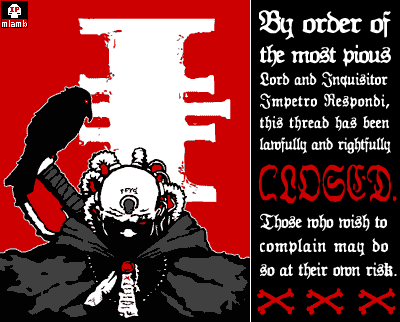
\includegraphics[width=400pt, height=322pt]{closedtopic.png}

It is possible that the topic may be reopened later. If necessary, some 
posts may be edited or hidden by the moderators, or the moderators 
decide that folks have cooled their heels enough to get a topic back on 
track. You can take it up with your forum moderator if you have issue 
with a closing, however please remain civil if you don't agree with 
what has been done. Flying off the handle will not help bring your 
point across.

\subsection{The Report Function}

Inevitably, members aren't going to agree on everything. And, the 
Internet being what it is, people often act is if it's okay to say 
whatever they want because there won't be any consequences. Or 
sometimes someone says something that you find offensive, or that you 
think is inappropriate in some way.

You'll be tempted to return fire, giving tit for tat or escalating.

The site doesn't need that. Remember, the mission of the site is to 
help each other to enjoy the hobby. It's difficult to do that when 
we're getting into spats with people we don't know.

Use the REPORT button when you see something that you think needs to be 
addressed. This will allow you to identify a potential problem to the 
staff, who will then take a look, discuss whether or not there is an 
issue that we need to handle, and then take whatever action we deem is 
appropriate.


\section{Projects \& Special Projects}

A variety of projects take place throughout the {\bnc}, 
ranging from the development of DIYs (in the Liber forums), member 
PLOGS (usually in the Forge forums, but often in the faction forums), 
to the development of special rules (usually in the Homegrown Rules 
forum). Some projects are more extensive, and we often refer to them as 
``special projects.''

Regardless of whether a project is ``regular'' or ``special'' and 
regardless of where it is conducted on the {\bnc} we've developed 
guidelines in the Special Projects forum here.

In an effort to maintain consistency and currency, we're not going to 
re-post those rules here. Simply follow the link for the definitive set 
of guidelines for projects.

\section{3D Printing}

  Wikipedia said:
\begin{quote}
3D printing is any of various processes in which material is joined or 
solidified under computer control to create a three-dimensional object, 
with material being added together (such as liquid molecules or powder 
grains being fused together).
\end{quote}

3D printing is a subset of additive manufacturing.

\section{Contacting the Administrators}


If you need to reach an Administrator for assistance, you can contact 
us via your normal e-mail at:

{\texttt{Brother Tyler -  TBD }}
\medskip
{\texttt{WarriorFish - TBD}}

\end{document}

